\documentclass[11pt]{article}
\usepackage[toc,page]{appendix}
\usepackage{amsmath, amssymb}
\usepackage[utf8]{inputenc}
\usepackage[T1]{fontenc}
\usepackage[style=apa,backend=biber]{biblatex}
%\usepackage{biblatex}
\addbibresource{references.bib}
\usepackage{graphicx}
\usepackage{tikz}
\usetikzlibrary{automata,positioning,shapes.geometric, arrows.meta, fit, backgrounds, calc, chains}
\graphicspath{./images/Easy_Pictures/SMR_MULT_Repackaging}%\usepackage{kpfonts}
\usepackage{float}
\usepackage[margin=1in]{geometry}
\usepackage{cancel}
\usepackage{epsfig}
\usepackage{tikz-3dplot}
\usepackage{darkmode}
\usepackage{dirtytalk}
\usepackage{longtable,booktabs,array}
\usepackage{calc} % for calculating minipage widths
\usepackage[utf8]{inputenc}
\usepackage[T1]{fontenc}
\usepackage{xcolor}
\usepackage{listings}


\usepackage{etoolbox}
\usepackage{hyperref}
\hypersetup{
    colorlinks=true,
    linkcolor=blue,
    filecolor=magenta,      
    urlcolor=cyan,
    pdftitle={Hermeneutic Calculator},
    citecolor=blue,
    }


\urlstyle{same}

\lstdefinestyle{htmlStyle}{
    language=HTML,
    basicstyle=\ttfamily\small,
    keywordstyle=\color{blue}\bfseries,
    commentstyle=\color{gray}\itshape,
    stringstyle=\color{red},
    breaklines=true,
    frame=single,
    numbers=left,
    numberstyle=\tiny\color{gray},
    columns=fullflexible,
}
\lstdefinelanguage{HTML}{
  keywords={<!DOCTYPE, html, head, title, body, h1, h2, h3, p, div, span, a, img, ul, li, table, tr, td, th, style, link, script},
  sensitive=true,
  comment=[l]{//},
  morecomment=[s]{/*}{*/},
  morestring=[b]',
  morestring=[b]"
}
\lstset{style=htmlstyle, language=html}
% Updated to explicitly pass the language option
%\lstinputlisting[style=htmlstyle, language=html]{./html/example.html}
%\usepackage{tocloft}

% Optional: define some custom colors
\definecolor{sliceRed}{RGB}{225,224,91} % matching "varyellow" from your code
\definecolor{linkYellow}{RGB}{255,215,0}  % a golden yellow
\tdplotsetmaincoords{70}{110}

\title{Addition Strategies: Counting On By Bases and then Ones (COBO)}
\author{Compiled by: Theodore M. Savich}


\begin{document}
\maketitle
\subsection*{Transcript}
Video from \textcite{Carpenter1999}. Strategy descriptions and examples adapted from \textcite{HackenbergCourseNotes}. 
\begin{itemize}
\item \textbf{Teacher:} Max  has  46  comic  books. For  his  birthday,  his  father  gives him  37  more  comic  books. How  many  comic  books  does  Max  have  now? 

\item \textbf{Lauren:} Forty-six  \ldots 
\item \textbf{Teacher:} He  gets  37  more  for  his  birthday. 
\item  \textbf{Lauren:} Ok. 46,  56, 66,  76,  77, 78,  79,  80,  81, 82,  83. It's  83. 
\item \textbf{Teacher:} Good  work.
\end{itemize}

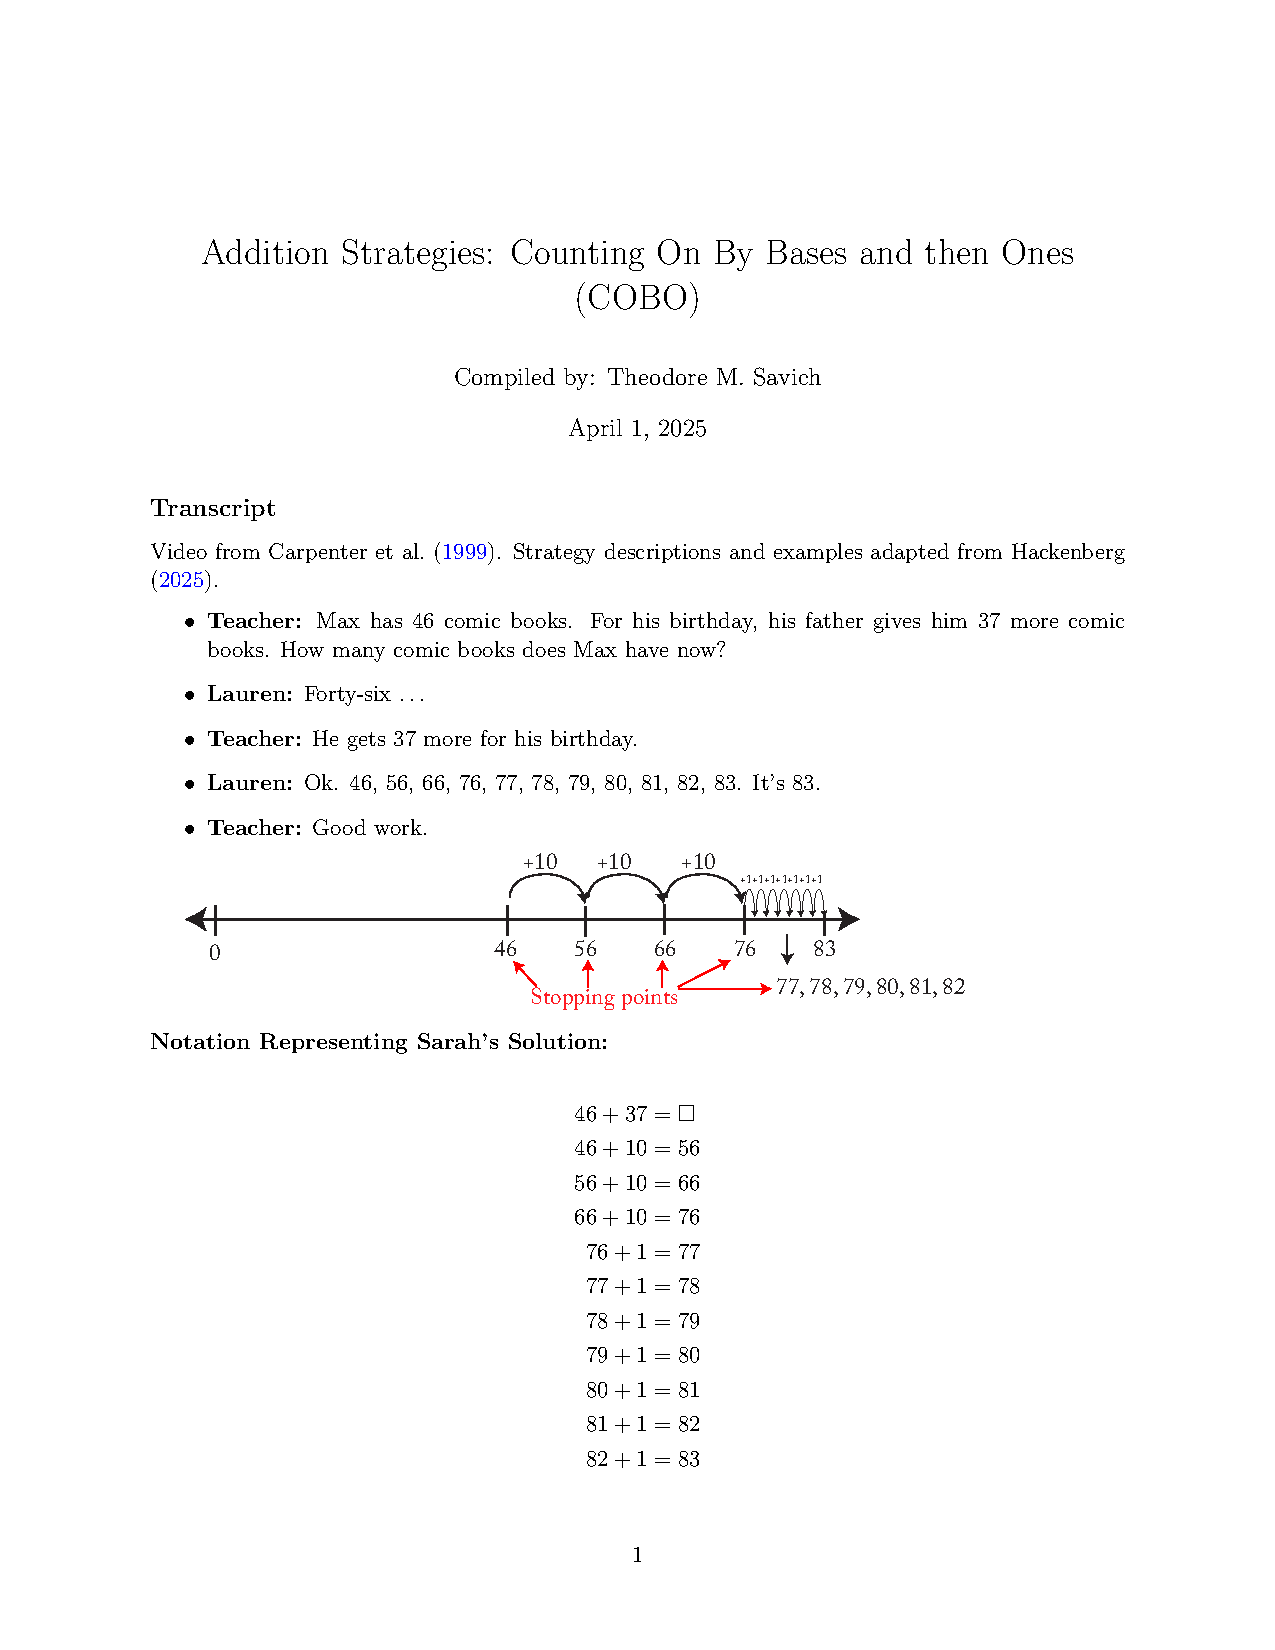
\includegraphics[width=.8\textwidth]{images/Easy_Pictures/SAR_ADD_COBO/PDF/SAR_ADD_COBO.pdf}

\noindent \textbf{Notation Representing Sarah's Solution:}

\begin{align*}
46 + 37 &= \Box \\
46+10 &= 56\\
56+10 &= 66\\
66+10 &= 76\\
76+1 &= 77\\
77+1 &= 78\\
78+1 &= 79\\
79+1 &= 80\\
80+1 &= 81\\
81+1 &= 82\\
82+1 &= 83\\
\end{align*}

\subsubsection*{Description of Strategy:}

 \textbf{Objective:} Description of Counting On by Bases and Then Ones (COBO)
 Begin with one of the numbers. Break the other number into its base units and its ones. Then, “count on” by adding each base unit one at a time, followed by each individual one.
 
 Why are number lines useful for demonstrating this strategy?
 COBO is essentially a jump strategy—you start at one number and make “jumps” equal to the other number’s base units, then add in the remaining ones. Number lines are ideal because they visually display jumps of varying lengths and directions. They serve as a picture of the process: a jump representing a full base is clearly larger (by a factor of the base) than a jump of a single unit.
 
 Good number line illustrations should:
\begin{itemize}
 \item Clearly represent the relative sizes of the jumps—each base jump should be exactly as many times larger than a single-unit jump as the base indicates, with all base jumps the same size and all one-unit jumps identical.
 \item Indicate the position of 0, or mark a break if that portion of the line isn’t drawn to scale.
 \item Use arrows to indicate direction—when adding, the jumps go to the right (or upward); when subtracting, they go to the left (or downward).
 \item Mark all landing points clearly—the numbers you would speak aloud when counting on by bases and then ones, just as Lauren demonstrated.
\end{itemize}

\subsection*{Counting On by Bases and Then Ones (COBO)}

\subsubsection*{Description of Strategy}
\begin{itemize}
    \item \textbf{Objective:} Start with one addend, add bases from the other addend one by one, then add ones one by one.
    \item \textbf{Example:} \(46 + 37\)
    \begin{itemize}
        \item Start at \(46\).
        \item Add tens one by one: \(46 \rightarrow 56 \rightarrow 66 \rightarrow 76\).
        \item Add ones one by one: \(76 \rightarrow 77 \rightarrow \ldots \rightarrow 83\).
    \end{itemize}
\end{itemize}

\subsubsection*{Automaton Type}
\textbf{Finite State Automaton (FSA) with Counters}:  
Counters are used to manage the repeated addition:
\begin{itemize}
    \item \textbf{BaseCounter:} Number of base units (e.g., tens) to add.
    \item \textbf{OneCounter:} Number of ones to add.
    \item \textbf{Sum:} The running total.
\end{itemize}

\subsubsection*{Automaton Definition SAR\_ADD\_COBO (Register Machine Model)}

To legitimately and deterministically represent the COBO strategy, we define a Register Machine with clearly defined, mutually exclusive conditions.

\textbf{M = (Q, V, \delta, q_0, F)}

\begin{itemize}
    \item \textbf{Q (States):} {$q_{start}, q_{initialize}, q_{add\_bases}, q_{add\_ones}, q_{accept}$}
    \item \textbf{V (Registers):} {A (Input), B (Input), Sum, BaseCounter, OneCounter}
    \item \textbf{Constants:} BaseUnit (e.g., 10)
\end{itemize}

\textbf{Transition Function (\delta):}

\begin{longtable}{|l|l|l|l|l|}
\hline
\textbf{Current State} & \textbf{Condition} & \textbf{Next State} & \textbf{Action} & \textbf{Interpretation} \\
\hline
\endhead
$q_{start}$ & (Input) & $q_{initialize}$ & Read A, Read B & Start. \\
\hline
$q_{initialize}$ & - & $q_{add\_bases}$ & Sum = A \newline BaseCounter = B // BaseUnit \newline OneCounter = B \% BaseUnit & Initialize Sum. Decompose B into Bases and Ones. \\
\hline
$q_{add\_bases}$ & \textbf{BaseCounter > 0} & $q_{add\_bases}$ & Sum = Sum + BaseUnit \newline BaseCounter = BaseCounter - 1 & Add one BaseUnit (Loop). \\
\hline
$q_{add\_bases}$ & \textbf{BaseCounter == 0} & $q_{add\_ones}$ & - & All bases added. Transition to adding ones. \\
\hline
$q_{add\_ones}$ & \textbf{OneCounter > 0} & $q_{add\_ones}$ & Sum = Sum + 1 \newline OneCounter = OneCounter - 1 & Add 1 (Loop). \\
\hline
$q_{add\_ones}$ & \textbf{OneCounter == 0} & $q_{accept}$ & Output Sum & All ones added. Accept. \\
\hline
\end{longtable}

\subsubsection*{Automaton Diagram for COBO}

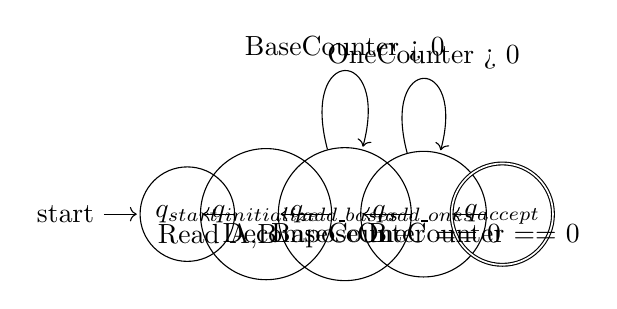
\begin{tikzpicture}[
    shorten >=1pt,
    on grid,
    auto,
    every state/.style={minimum size=1.2cm}
]
    % Define nodes
    \node[state, initial] (start) {$q_{start}$};
    \node[state, right=of start] (initialize) {$q_{initialize}$};
    \node[state, right=of initialize] (add_bases) {$q_{add\_bases}$};
    \node[state, right=of add_bases] (add_ones) {$q_{add\_ones}$};
    \node[state, accepting, right=of add_ones] (accept) {$q_{accept}$};

    % Transitions
    \path[->]
        (start) edge node {Read A,B} (initialize)
        (initialize) edge node {Decompose B} (add_bases)
        (add_bases) edge[loop above] node {BaseCounter > 0} (add_bases)
        (add_bases) edge node {BaseCounter == 0} (add_ones)
        (add_ones) edge[loop above] node {OneCounter > 0} (add_ones)
        (add_ones) edge node {OneCounter == 0} (accept);
\end{tikzpicture}

\subsubsection*{Python Implementation and Test}

The following Python code implements the corrected COBO automaton.

\begin{lstlisting}[language=Python]
import pandas as pd

class COBOAutomaton:
    """
    A Register Machine model simulating the 'Counting On By Bases and then Ones' (COBO) strategy.
    """
    def __init__(self, A, B, Base=10):
        self.A = A
        self.B = B
        self.BaseUnit = Base

        # Registers for internal computation
        self.Sum = 0
        self.BaseCounter = 0
        self.OneCounter = 0

        # State
        self.state = 'q_start'
        self.history = []

    def _record_history(self, action, interpretation):
        self.history.append({
            'State': self.state,
            'Sum': self.Sum,
            'BaseCounter': self.BaseCounter,
            'OneCounter': self.OneCounter,
            'Action': action,
            'Interpretation': interpretation,
        })

    def transition(self, next_state):
        self.state = next_state

    def run(self):
        while self.state not in ['q_accept', 'q_error']:
            if self.state == 'q_start':
                self.execute_start()
            elif self.state == 'q_initialize':
                self.execute_initialize()
            elif self.state == 'q_add_bases':
                self.execute_add_bases()
            elif self.state == 'q_add_ones':
                self.execute_add_ones()
            else:
                self.transition('q_error')
                break
        return self.Sum

    def execute_start(self):
        """q_start: Read inputs."""
        self._record_history(f"Read A={self.A}, B={self.B}", "Start.")
        self.transition('q_initialize')

    def execute_initialize(self):
        """q_initialize: Initialize Sum and decompose B."""
        self.Sum = self.A
        # Decomposition (Assuming this skill is prerequisite for COBO)
        self.BaseCounter = self.B // self.BaseUnit
        self.OneCounter = self.B % self.BaseUnit

        action = f"Sum=A; Decompose B ({self.B})"
        interpretation = f"Initialize Sum to {self.A}. {self.BaseCounter} Bases, {self.OneCounter} Ones."
        self._record_history(action, interpretation)
        # Proceed to the base addition phase
        self.transition('q_add_bases')

    def execute_add_bases(self):
        """q_add_bases: Iteratively add BaseUnits."""
        # Condition: BaseCounter > 0 (Loop Iteration)
        if self.BaseCounter > 0:
            prev_sum = self.Sum
            self.Sum += self.BaseUnit
            self.BaseCounter -= 1

            action = f"Sum += {self.BaseUnit}; BaseCounter -= 1"
            interpretation = f"Count on by base: {prev_sum} -> {self.Sum}."
            self._record_history(action, interpretation)
            # Stay in the same state
        # Condition: BaseCounter == 0 (Loop Exit)
        else:
            self._record_history("BaseCounter == 0", "All bases added. Transition to adding ones.")
            self.transition('q_add_ones')

    def execute_add_ones(self):
        """q_add_ones: Iteratively add Ones."""
        # Condition: OneCounter > 0 (Loop Iteration)
        if self.OneCounter > 0:
            prev_sum = self.Sum
            self.Sum += 1
            self.OneCounter -= 1

            action = "Sum += 1; OneCounter -= 1"
            interpretation = f"Count on by one: {prev_sum} -> {self.Sum}."
            self._record_history(action, interpretation)
            # Stay in the same state
        # Condition: OneCounter == 0 (Loop Exit)
        else:
            self._record_history("OneCounter == 0", "All ones added. Accept.")
            self.transition('q_accept')

    def display_history(self):
        print(f"\n--- COBO Execution History ({self.A} + {self.B}) ---")
        df = pd.DataFrame(self.history)
        print(df.to_markdown(index=False))

# Test the automaton with Lauren's example: 46 + 37.
cobo_automaton = COBOAutomaton(A=46, B=37)
result = cobo_automaton.run()
cobo_automaton.display_history()
print(f"\nFinal Result: {result}")
\end{lstlisting}

\subsubsection*{Execution Trace (46 + 37):}
\begin{verbatim}
--- COBO Execution History (46 + 37) ---
| State          |   Sum |   BaseCounter |   OneCounter | Action                       | Interpretation                                    |
|:---------------|------:|--------------:|-------------:|:-----------------------------|:--------------------------------------------------|
| q_start        |     0 |             0 |            0 | Read A=46, B=37              | Start.                                            |
| q_initialize   |    46 |             3 |            7 | Sum=A; Decompose B (37)      | Initialize Sum to 46. 3 Bases, 7 Ones.            |
| q_add_bases    |    56 |             2 |            7 | Sum += 10; BaseCounter -= 1  | Count on by base: 46 -> 56.                       |
| q_add_bases    |    66 |             1 |            7 | Sum += 10; BaseCounter -= 1  | Count on by base: 56 -> 66.                       |
| q_add_bases    |    76 |             0 |            7 | Sum += 10; BaseCounter -= 1  | Count on by base: 66 -> 76.                       |
| q_add_bases    |    76 |             0 |            7 | BaseCounter == 0             | All bases added. Transition to adding ones.       |
| q_add_ones     |    77 |             0 |            6 | Sum += 1; OneCounter -= 1    | Count on by one: 76 -> 77.                        |
| q_add_ones     |    78 |             0 |            5 | Sum += 1; OneCounter -= 1    | Count on by one: 77 -> 78.                        |
| q_add_ones     |    79 |             0 |            4 | Sum += 1; OneCounter -= 1    | Count on by one: 78 -> 79.                        |
| q_add_ones     |    80 |             0 |            3 | Sum += 1; OneCounter -= 1    | Count on by one: 79 -> 80.                        |
| q_add_ones     |    81 |             0 |            2 | Sum += 1; OneCounter -= 1    | Count on by one: 80 -> 81.                        |
| q_add_ones     |    82 |             0 |            1 | Sum += 1; OneCounter -= 1    | Count on by one: 81 -> 82.                        |
| q_add_ones     |    83 |             0 |            0 | Sum += 1; OneCounter -= 1    | Count on by one: 82 -> 83.                        |
| q_add_ones     |    83 |             0 |            0 | OneCounter == 0              | All ones added. Accept.                           |
\end{verbatim}

\printbibliography
\end{document}